\chapter{\uppercase{Reactor Neutrinos}}

Fission of isotopes used in reactor fuel cause a chain reaction that results in several  $\beta$ decays, creating electron antineutrinos, $\bar{\nu_{e}}$.
For this reason, nuclear reactors are a powerful and pure source of $\bar{\nu_{e}}$, meaning that there are no reactions taking place in the reactor that create the other active neutrino flavors.
The first neutrino was discovered using the nuclear reactor at the Savannah River Plant due to its continuous flux of $\bar{\nu_{e}}$ and the ability to get close to the core.
A host of current neutrino experiments are located at reactors, making it important to understand the reactor neutrino flux and spectrum. 

\section{Production of Reactor Neutrinos}

Nuclear reactors are powered by the fission of uranium and plutonium isotopes in their cores. 
Specifically, in a power reactor, 99.9\% of the power comes from the fission of $^{235}$U, $^{239}$Pu, $^{241}$Pu, and $^{238}$U isotopes and the subsequent beta decays.
The reaction begins with a neutron colliding with a nucleus of one of the isotopes. 
This causes the nucleus to split into two neutron-rich fragments, usually of unequal mass, creating an unstable system.
In order to reach stability neutrons have to transform into protons, a process accomplished through $\beta$ decay, see Figure~\ref{fig:nucchart}.
On average each daughter $\beta$ decays three times to reach stability.
Each beta decay produces an electron and corresponding electron antineutrino. 
In general a nuclear reactor will produce $\sim 6 \times 10^{20}~\bar{\nu_e}$ per GW of thermal energy power \cite{HayesVogel}.

\begin{figure}[h]
	\centering
	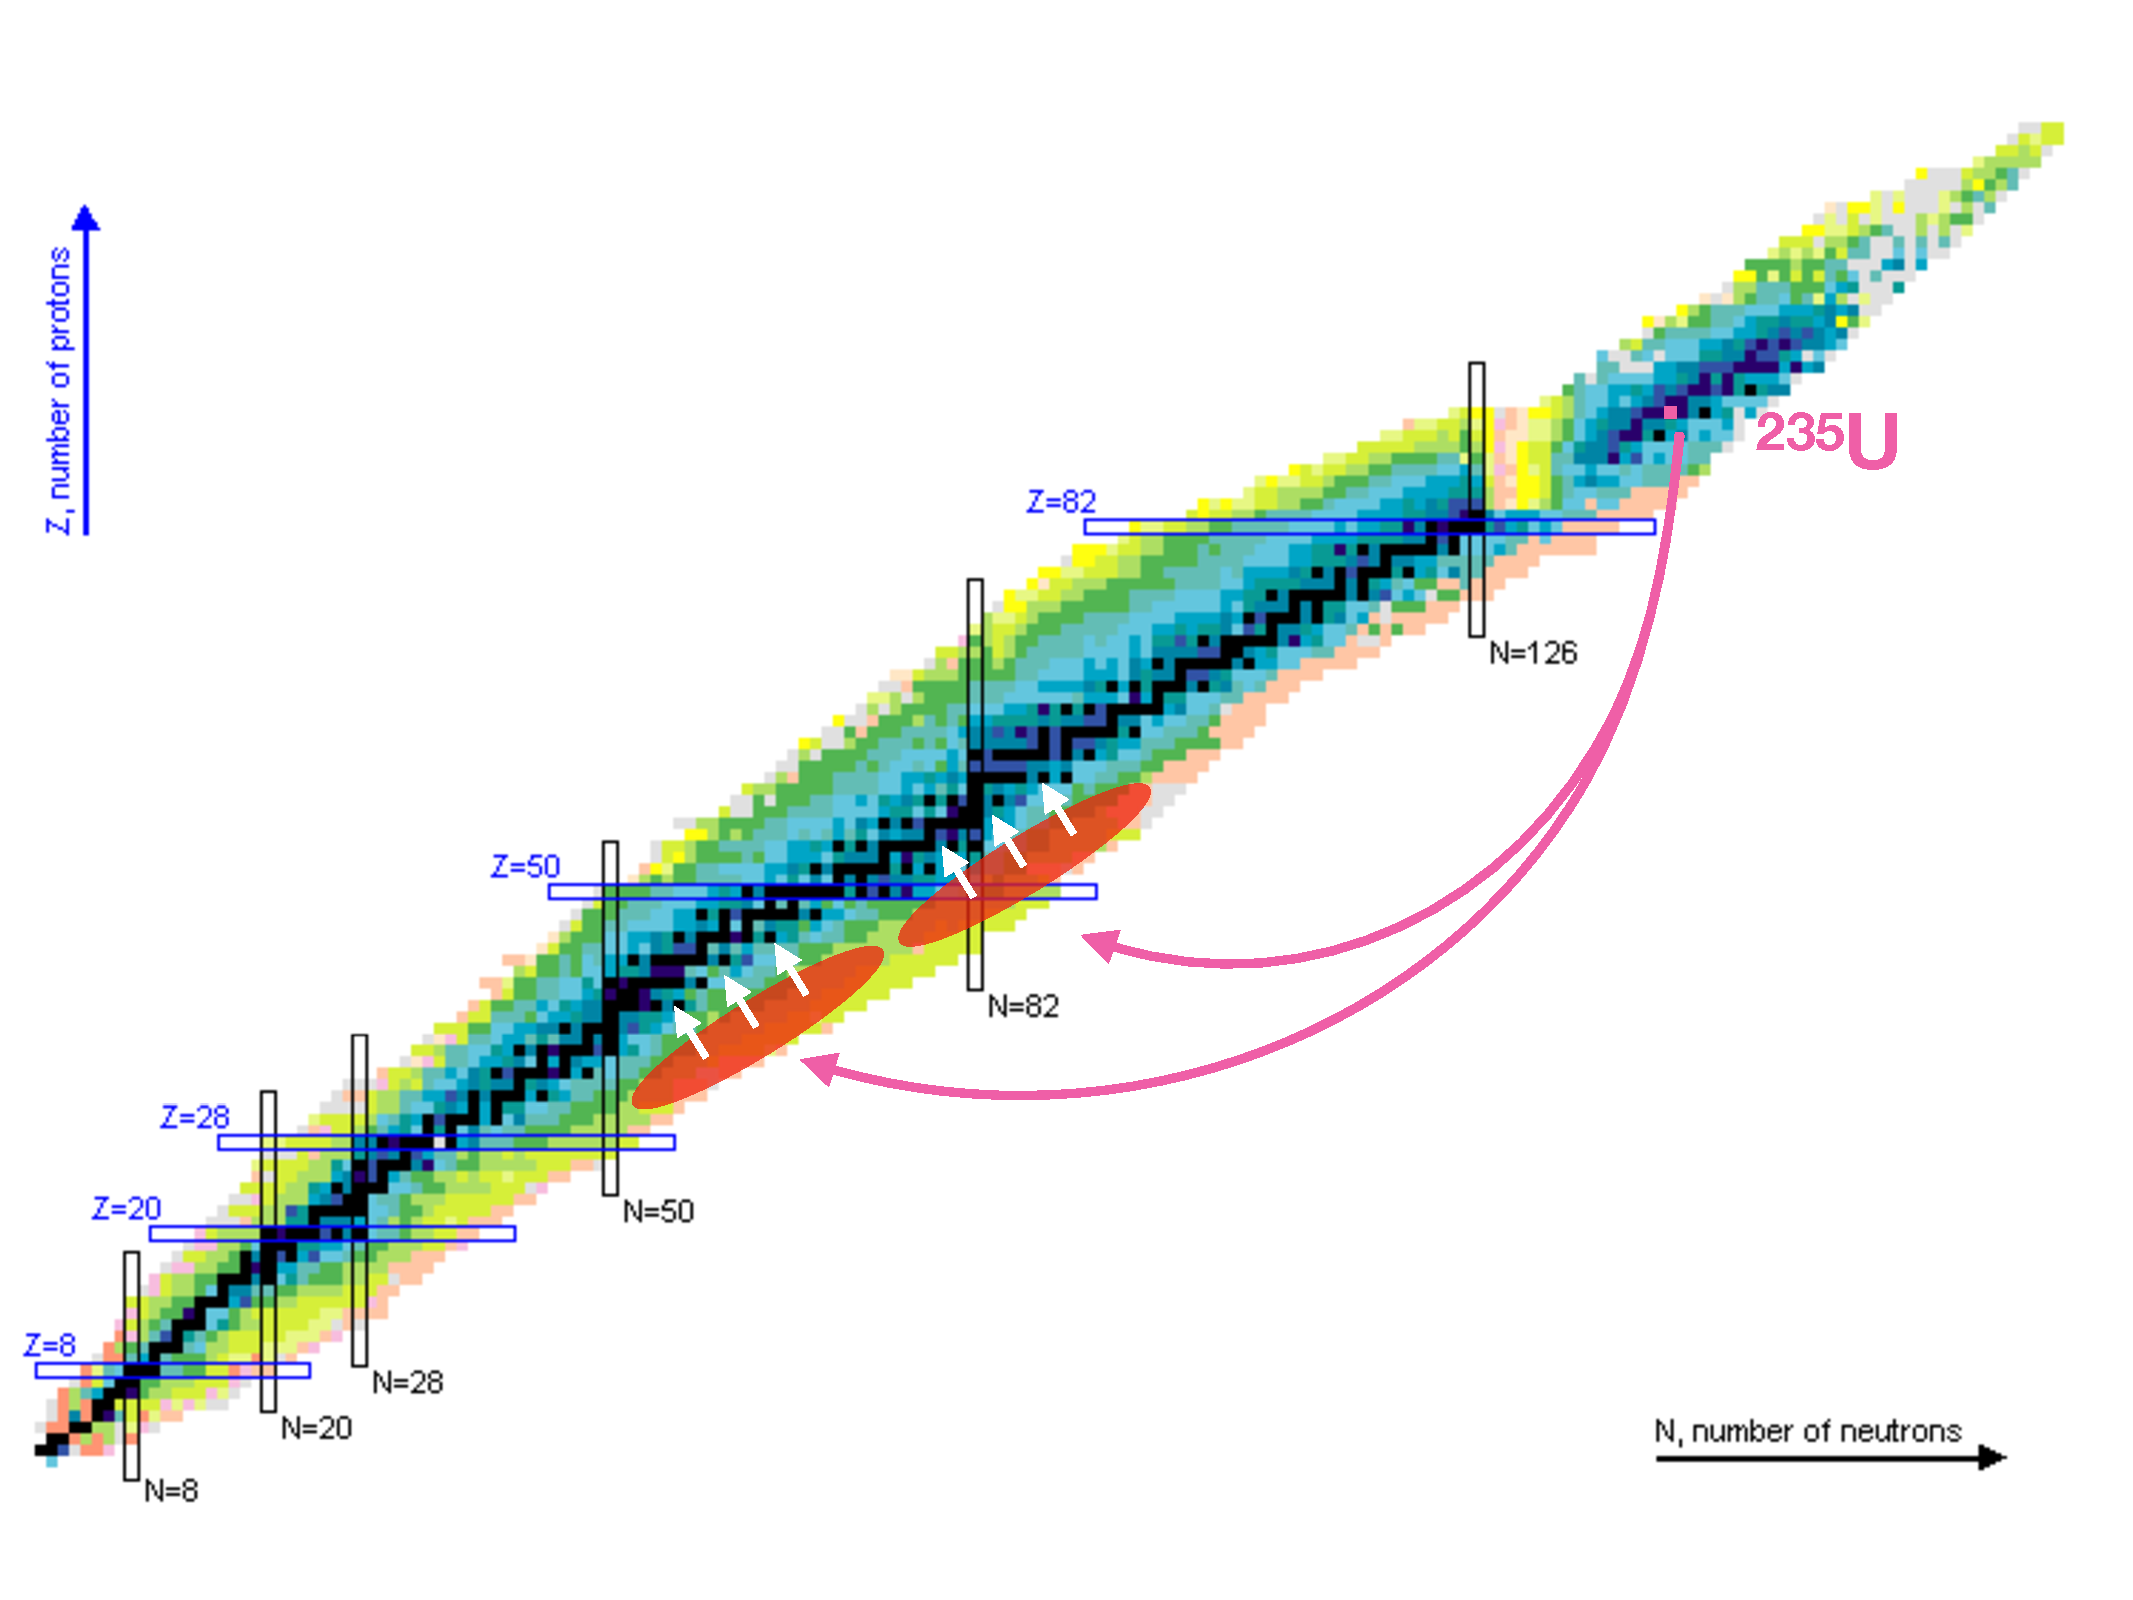
\includegraphics[width=0.7\linewidth]{tex/3-reactorneutrinos-images/NuclideChart_U235}
	\caption{A schematic of the fission of $^{235}$U \cite{NucChart}. After collision with a neutron $^{235}$U will split into two unstable, neutron-rich nuclei (arrows, pink) which will then $\beta$ decay (arrows, white) until stable.}
	\label{fig:nucchart}
\end{figure}


\section{Measuring the Reactor Antineutrino Flux and Spectrum}

The total $\bar{\nu_{e}}$ flux, $S(E_\nu)$, produced by a nuclear reactor can be expressed as the sum over the spectra of the dominant fissioning isotopes,
\begin{equation}
	S(E_\nu) = \frac{W_{th}}{\sum_{i}(f_i/F)e_i}\sum_{i}\frac{f_i}{F}\left(\frac{dN_i}{dE_\nu}\right) ,
\end{equation}
where $f_i/F$ is the fission fraction for each given isotope $i$, $W_{th}$ is the reactor thermal energy, $e_i$ is the 
average energy released per fission by each isotope, and $dN_i/dE_\nu$ is the cumulative $\bar{\nu_e}$ spectrum of $i$ normalized per fission \cite{HayesVogel}.

There are two methods used to determine the $\bar{\nu_e}$ spectrum, \textit{ab initio} summation and electron spectrum conversion.
In the \textit{ab initio} approach the spectrum is determined by summing the contributions of all $\beta$-decay branches of all fission fragments,
\begin{equation}
	\frac{dN_i}{dE_{\bar{\nu}}} =  \sum_{n}Y_n(Z,A,t)\sum_{i}b_{n,i}(E^i_0)P_{\bar{\nu}}(E_{\bar{\nu}},E^i_0,Z) ,
\end{equation}
where $Y_n(Z,A,t)$ is the number of $\beta$ decays of the fission fragment $Z, A$ at time $t$, $b_{n,i}(E^i_0)$ are the branching ratios with endpoint energies $E^i_0$, and $P_{\bar{\nu}}(E_{\bar{\nu}},E^i_0,Z)$ is the normalized $\bar{\nu_e}$ spectrum for the branch $n, i$ \cite{HayesVogel}.
This method relies on nuclear databases, such as the Evaluated Nuclear Data File (ENDF) \cite{ENDF} and Joint Evaluated Fission and Fusion Data Library (JEFF) \cite{JEFF} for fission yields of daughter products, and the Evaluated Nuclear Structure Data File (ENSDF) \cite{ENSDF} for spectra, branching ratios and endpoint energies.
The antineutrino spectrum for the four main reactor isotopes calculated using \textit{ab initio} summation was done in~\cite{HayesVogel} and the result can be seen in Figure~\ref{fig:spectrum}. 

Though seemingly straightforward, this approach comes with some caveats.
The sheer number of daughter isotopes ($>$1000) and individual $\beta$ decay branches ($>$6000) make the summation non-trivial.
This, along with the fact that not all branching ratios are known, and that the fission yields have been determined by several different database groups but don't always agree and have large uncertainties bring into question the validity of using only this method. 

\begin{figure}[t]
	\centering
	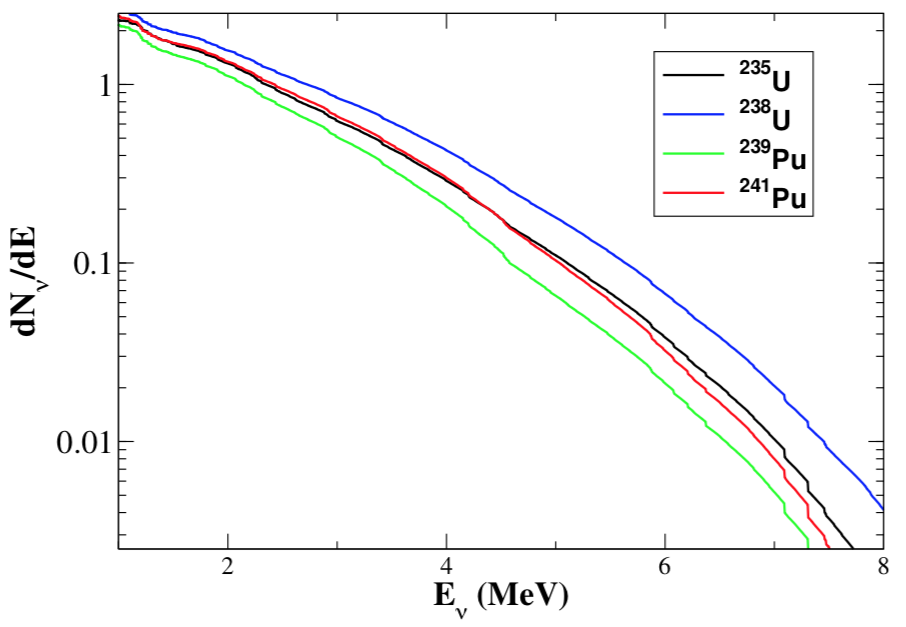
\includegraphics[width=0.65\linewidth]{tex/3-reactorneutrinos-images/Spectrum}
	\caption{The $\bar{\nu_e}$ spectrum predicted by the summation method using the JEFF-3.1.1 database fission fragment yields and the ENDF/B-VII.1 decay library \cite{HayesVogel}.}
	\label{fig:spectrum}
\end{figure}

The other approach to determining the $\bar{\nu_{e}}$ spectrum, sometimes called the conversion method, relies on converting a measured electron spectrum into an antineutrino spectrum. 
A set of virtual end-point energies, $E^i_0$, are defined by binning the total measured beta spectrum over an energy grid. 
The total spectrum is fit with individual beta spectra in terms of their amplitudes, $a_i$, for each virtual end-point energy, 
\begin{equation}
	\frac{dN_i}{dE_e} = \sum_{i}a_iP(E,E^i_0,Z).
\end{equation}
The conversion to the antineutrino spectrum is then accomplished by replacing the energy $E_e$ in each branch by $E_0 - E_{\bar{\nu}}$, because the electron and the $\bar{\nu_e}$ share the total energy of each $\beta$-decay branch.
The flux per fission is then given as the sum of $\bar{\nu_e}$ spectrum converted from each virtual $\beta$ branch,
\begin{equation}
	\frac{dN_i}{dE_{\bar{\nu}}} = \sum_{i}a_iP(E^i_0-E,E^i_0).
\end{equation}

%\begin{figure}
%	\centering
%	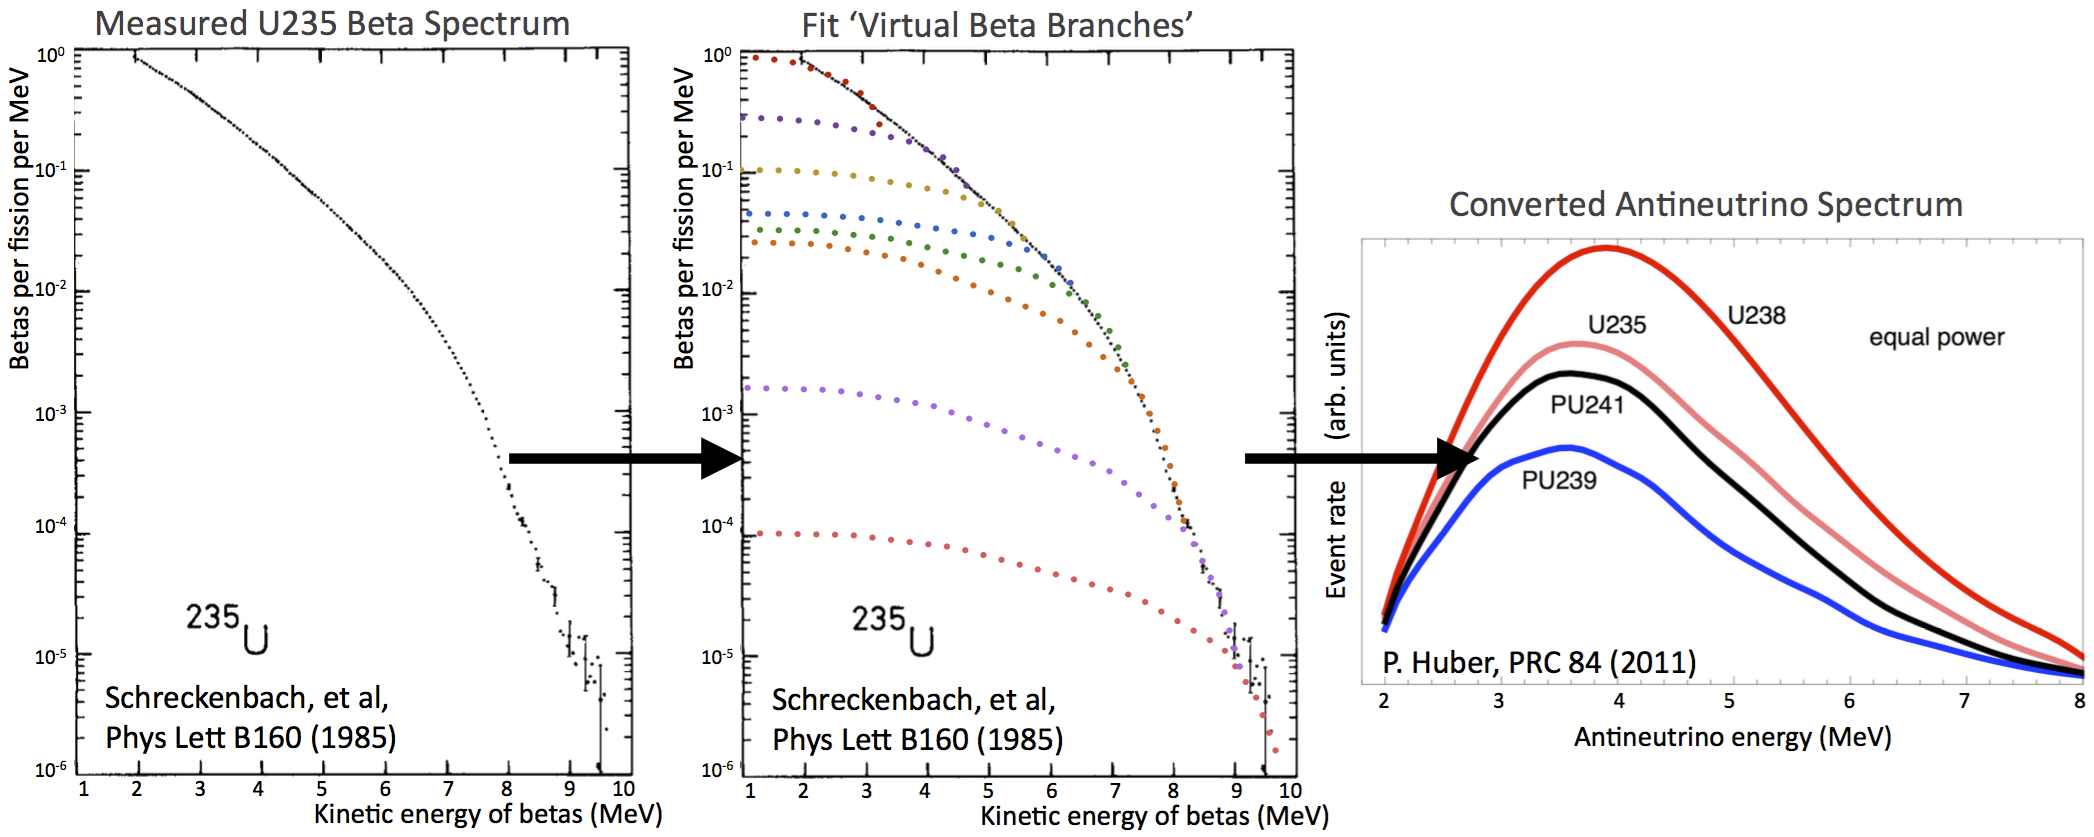
\includegraphics[width=0.7\linewidth]{tex/3-reactorneutrinos-images/betaspecconversion_fixed}
%	\caption{}
%	\label{fig:betaspecconversionfixed}
%\end{figure}

The electron spectra for $^{235}$U, $^{239}$Pu, and $^{241}$Pu were measured at the Institut
Laue-Langevin (ILL) reactor in Grenoble, France in the 1980s \cite{VonFeilitzsch:1982jw,Schreckenbach:1985ep,Hahn:1989zr}, while the spectrum of $^{238}$U was more recently (2014) measured at the neutron source FRMII in Garching, Germany \cite{Haag:2013raa}.
The ILL measurements, along with a prediction of the $^{238}$U $\bar{\nu_{e}}$ spectrum using the summation method by Vogel \cite{PhysRevC.24.1543}, became known as the ``ILL-Vogel" flux model and was the main model used until 2011.

In 2011 Mueller \textit{et al.} improved the prediction of the reactor antineutrino spectra by employing a method that combined information from the nuclear databases and the measured electron spectra from ILL \cite{Mueller}. 
This was followed by a further improvement by Huber who applied higher order corrections making use of the conversion method and minimizing the use of the databases as much as possible \cite{Huber}.

Though much work has been done to accurately model the reactor antineutrino spectra both methods are subject to uncertainties in the subdominant corrections to beta-decay. This includes radiative, weak magnetism, and finite size corrections along with uncertainties in the spectrum shape of forbidden transitions which are summarized in~\cite{HayesVogel}. 

Besides the model uncertainties there are also experimental uncertainties that arise from knowing the thermal power of the reactor, its time-dependent fuel composition, and the fission energies of the dominant isotopes.
All of these uncertainties result in a 10-20\% relative uncertainty on the reactor antineutrino spectra using the \textit{ab initio} method and $\sim$5 \% uncertainty on the conversion approach \cite{Qian:2018wid}.



\section{Detection of Reactor Neutrinos}

Though there are several methods that can be used to detect reactor neutrinos, including charge-current ($\bar{\nu_e} + d \rightarrow n + n + e^+$), neutral-current ($\bar{\nu_e} + d \rightarrow n + p + \bar{\nu_e}$), and antineutrino-electron elastic scattering ($\bar{\nu_e} + e^- \rightarrow \bar{\nu_e} + e^-$) \cite{SuperKOsc,SNO}, the one employed by most experiments is IBD ($\bar{\nu_e} + p \rightarrow e^+ + n$).
The IBD reaction threshold, in the frame in which the proton is at rest, is given by
\begin{equation}
	E_{\textrm{thresh}} = \frac{(M_n + m_e)^2 - M_p^2}{2M_p} \approx 1.806~\textrm{MeV},
\end{equation}
where $M_n, ~m_e,$ and $M_p$ are the mass of the neutron, electron, and proton respectively and the mass of the antineutrino is neglected.

The cross section of this reaction, to zeroth order in $1/M$ (where $M$ is the nucleon mass) can be written as
\begin{equation}
\sigma^{(0)} = \frac{2\pi^2/m_e^2}{{f^R}\tau_n}E_e^{(0)}p_e^{(0)} \approx 9.52 \times \left(\frac{E_e^{(0)}p_e^{(0)}}{\textrm{MeV}^2}\right) \times 10^{-44}\textrm{cm}^2,
\end{equation}
where $\tau_n$ is the neutron decay lifetime, $f^R = 1.7152$ is the neutron decay phase-space factor that includes the Coulomb, weak magnetism, recoil, and outer radiative corrections, and $E_e$ and $p_e$ are the energy momentum of the final-state positron \cite{HayesVogel}.
At reactor energies, though, first order corrections in $1/M$ should be included \cite{Vogel:1999zy} and the resulting IBD cross section as a function of neutrino energy can be seen in Figure~\ref{fig:vogel-fig02}.


An IBD event is selected by a pair of coincident signals consisting of a positron ionization and annihilation as the prompt signal and a time delayed neutron capture on a proton or nucleus as the delay signal. 
The positron, carrying most of the $\bar{\nu_{e}}$ energy, will produce two 511 keV gammas as a result of the pair annihilation, which means that the minimum energy of the prompt signal is 1.022 MeV.
These two gammas will Compton scatter initiating a release of more electrons creating scintillation light.
The positron ionization, annihilation, and Compton scattering are detected as one signal, giving the prompt energy, $E_{\textrm{prompt}}$.

The neutrino energy, $E_{\bar{\nu_{e}}}$, can then be calculated from this prompt signal as 
\begin{equation}
\begin{split}
	E_{\bar{\nu_{e}}} &= E_{\textrm{prompt}} + (1.8~\textrm{MeV} - 1.022~\textrm{MeV}) + T_n \\
			&\approx E_{\textrm{prompt}} + 0.78~\textrm{MeV},
\end{split}
\end{equation}
where $T_n$ is the kinetic energy of the recoil neutron which is much smaller than the energy of the neutrino and can therefore be ignored in most cases. 
The IBD cross-section increases with energy, whereas the $\bar{\nu_{e}}$ spectrum decreases with energy creating a detected antineutrino energy spectrum that peaks around 3.8 MeV and decreases to zero above $\sim$8 MeV, as seen in Figure~\ref{fig:vogel-fig02}. 
In addition to great background rejection and good reconstruction of the neutrino energy, the IBD method of detecting neutrinos also allows the use of liquid scintillators and water as detection mediums. 

\begin{figure}[!t]
	\centering
	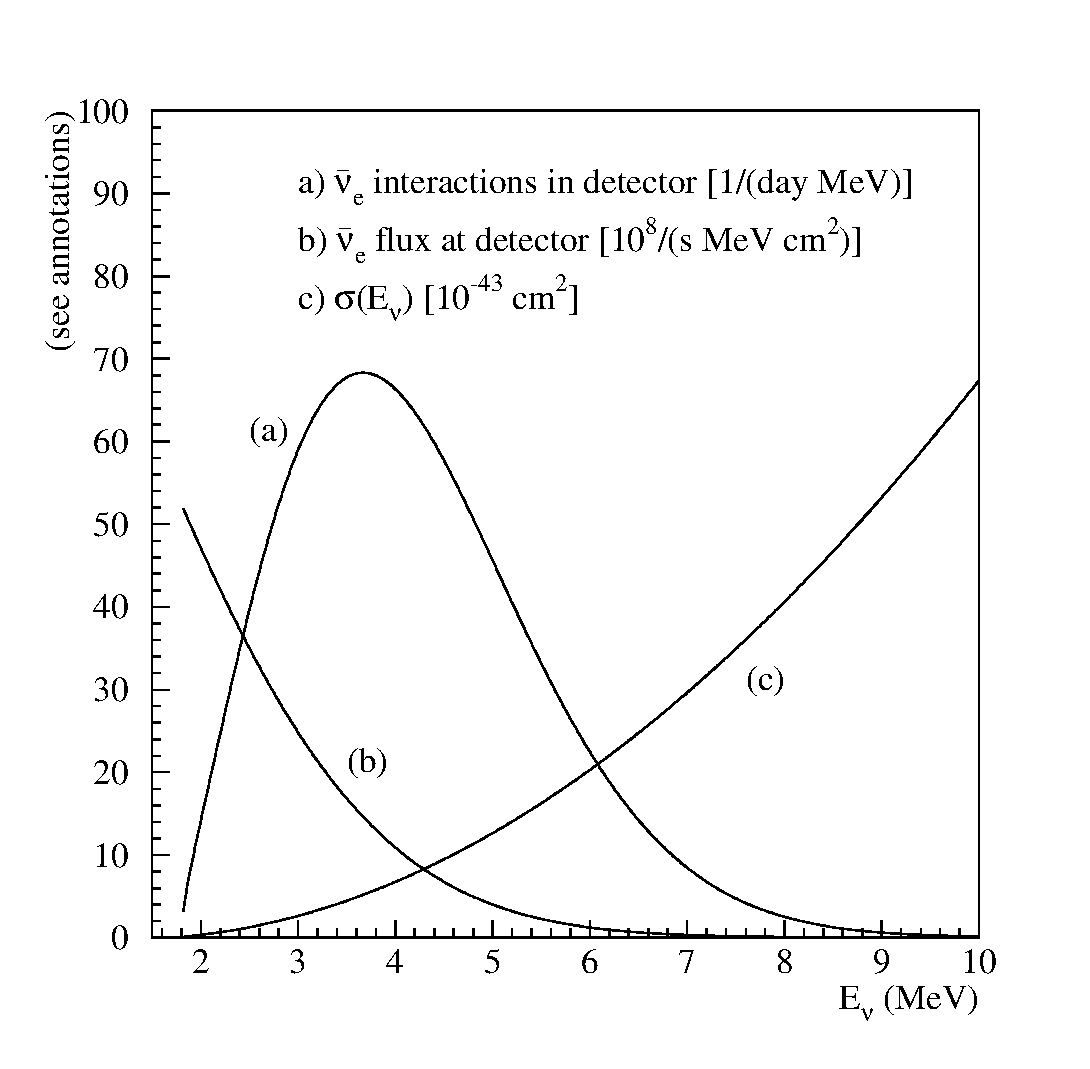
\includegraphics[width=0.55\linewidth]{tex/3-reactorneutrinos-images/vogel-fig02}
	\caption{The IBD spectrum (curve (a)) measured by a 12-ton fiducial mass detector located 0.8 km from a 12-GW$_{th}$ power reactor along with the reactor flux (curve (b)) and IBD cross section (curve (c)) as a function of energy \cite{PDG}.}
	\label{fig:vogel-fig02}
\end{figure}


\section{The Reactor Antineutrino Anomaly}

Several experiments have, and continue to use reactor antineutrinos to search for neutrino oscillation. 
A reactor neutrino disappearance $P(\bar{\nu_{e}} \rightarrow \bar{\nu_{e}})$ experiment can measure the mixing angle $\theta_{13}$ by placing their detector near the first maximum of $\sin^2\left(\frac{\Delta m^2_{31}L}{4E}\right)$, for which the amplitude of the oscillation gives $\sin^22\theta_{13}$ (recall Eq.~\ref{eq:oscprob}).
In the late 1990's the CHOOZ \cite{Apollonio:1999ae,Apollonio:2002gd} and Palo Verde \cite{Boehm:2001ik} experiments attempted to do this by placing their detectors at a baseline of $\sim$1 km from a nuclear reactor, but neither observed oscillations.

Though unsuccessful in making a measurement of $\theta_{13}$, the work of these collaborations helped to inform the decisions of successor experiments, Daya Bay in China, RENO in Korea, and Double Chooz in France. 
It should also be noted here that the Kamioka Liquid scintillator Anti-Neutrino Detector (KamLAND) experiment was successful in making measurements of $\theta_{12}$ and $\Delta m^2_{12}$  by placing their detectors at a long baseline of, on average, 180 km \cite{Eguchi:2002dm, Araki:2004mb}.

The Daya Bay Reactor Neutrino Experiment was located at the Daya Bay nuclear reactor power plant in southern China that consists of six 2.9 GW$_{th}$ reactors. 
They employed antineutrino detectors (AD) near and far from the reactors so that they could make a relative comparison of rates in order to suppress the reactor flux uncertainties \cite{An:2015qga,DayaBayAnomaly}.
The IBD yield measured for each AD is shown in Figure~\ref{fig:dayabayflux} and it can be seen that, after correcting for small variations of fission fractions among the different sites, all rates are consistent with each other. Though results between detectors agree, the disagreement between the experimental results and most recent model calculations (Huber+Mueller) is significant. 

\begin{figure}[!t]
	\centering
	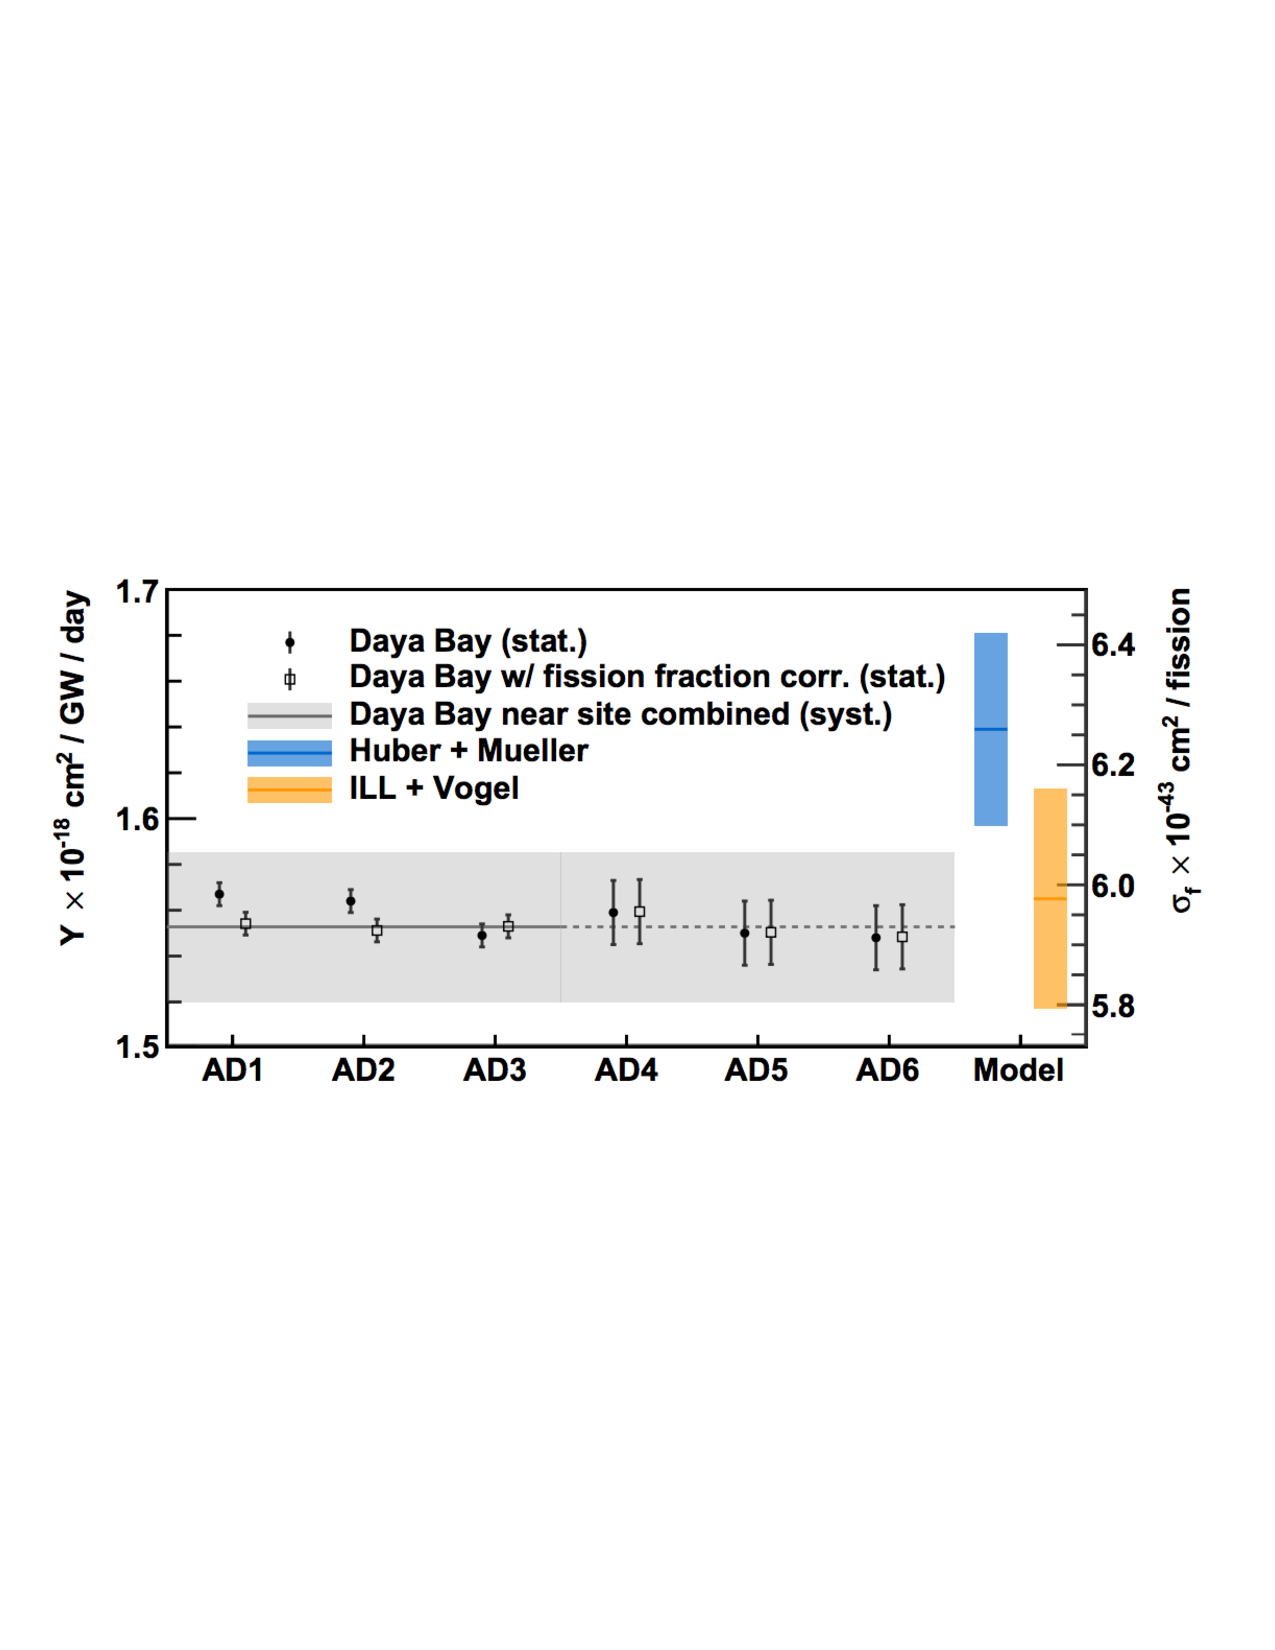
\includegraphics[width=0.7\linewidth]{tex/3-reactorneutrinos-images/DayaBayFlux}
	\caption{Rate of reactor antineutrino candidate events in Daya Bay's six detectors \cite{DayaBayAnomaly}. The average of the three near detectors is shown as the gray line, extended though the far detectors as a dotted gray line. Also shown are the rates predicted using the Huber+Mueller (blue) and ILL+Vogel (orange) models.}
	\label{fig:dayabayflux}
\end{figure}

\begin{figure}[!t]
	\centering
	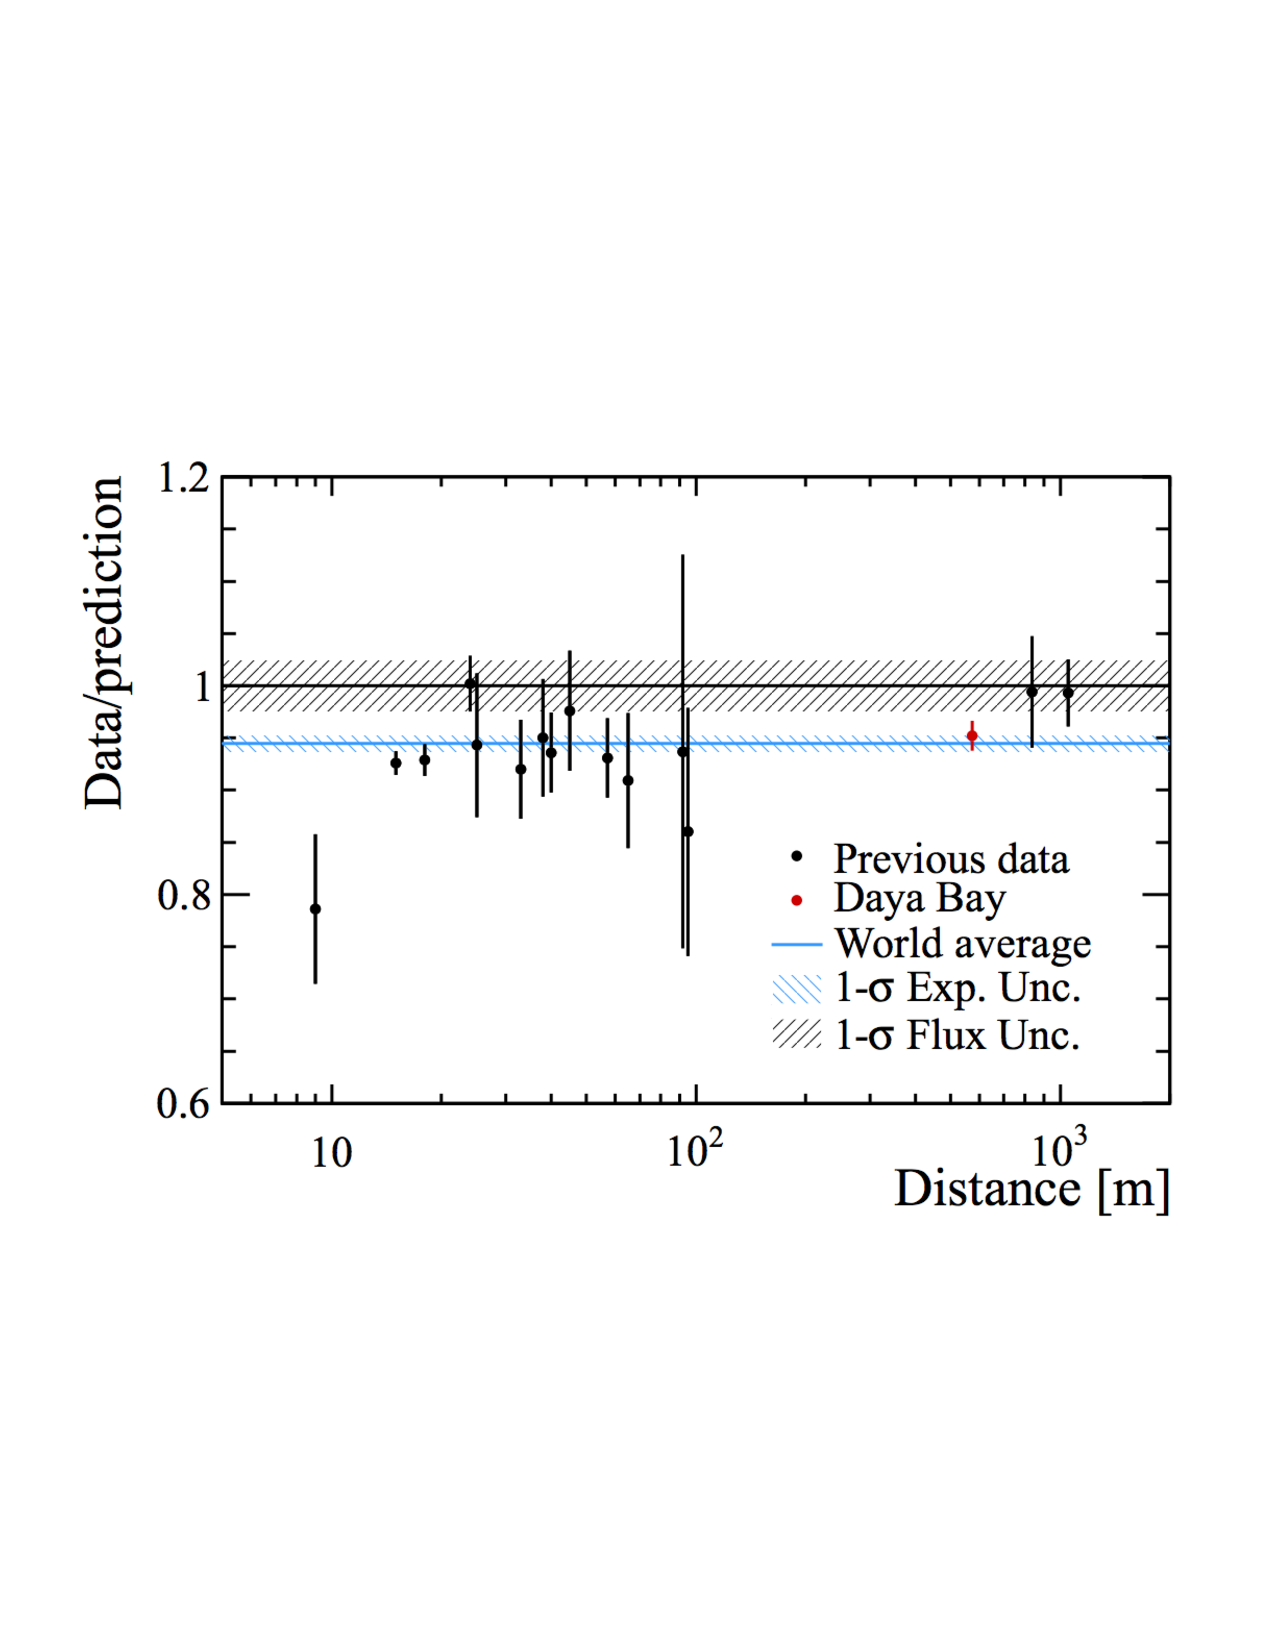
\includegraphics[width=0.6\linewidth]{tex/3-reactorneutrinos-images/WorldAvgFlux}
	\caption{The measured reactor $\bar{\nu_{e}}$ rate, normalized to the Huber+Mueller model prediction, as a function of distance from the reactor \cite{DayaBayFlux2018}. The rate is corrected for 3-flavor neutrino oscillations at each baseline. The blue shaded region represents the global average and its 1$\sigma$ uncertainty. The 2.7$\sigma$ model uncertainty is shown as a band around unity.}
	\label{fig:worldavgflux}
\end{figure}

In order to obtain a wider picture, the Daya Bay average IBD yield at the flux-weighted baseline (573 m) of the two near detector sites was compared to measurements from nineteen other short-baseline ($<$1000 m) experiments as shown in Figure~\ref{fig:worldavgflux}. 
The global average, including the most recent Daya Bay calculation, results in a ratio of measured to expected yield of 0.945 $\pm$ 0.007 (exp.) $\pm$ 0.023 (model) with respect to the Huber+Mueller model, a $\sim$6\% deficit \cite{DayaBayFlux2018}.
If the model uncertainty is to be trusted this ratio suggests reactor $\bar{\nu_{e}}$ disappearance as close as L$<$10 m, a phenomenon not covered in the standard 3-flavor neutrino mixing model \cite{HayesVogel}.  
This discrepancy has been labeled the ``Reactor Antineutrino Anomaly" (RAA). 

One hypothesis for explaining the reactor anomaly is that reactor neutrinos are oscillating into a new type of neutrino, a sterile neutrino. 
A sterile neutrino does not take part in weak interactions except those induced by mixing with the three generations of active neutrinos.
Anomalous results that might be explained by sterile neutrinos are also not confined to reactor experiments.  
Specifically, the Liquid Scintillation Neutrino Detector (LSND)  measured an excess of $\bar{\nu_{e}}$ ($>$3$\sigma$) events \cite{Aguilar:2001ty} along with excesses measured by the Mini Booster Neutrino Experiment (MiniBooNE) of $\nu_{e}$ (3.4$\sigma$) and $\bar{\nu_{e}}$ (2.8$\sigma$) \cite{Aguilar-Arevalo:2013pmq}.
Two solar neutrino detectors, the Soviet–American Gallium Experiment (SAGE) and Gallium Experiment (GALLEX), have observed a deficit in electron neutrinos produced by intense artificial $^{51}$Cr and $^{37}$Ar radioactive sources at a significance of 3$\sigma$ \cite{Giunti:2010zu}.

\begin{figure}[!t]
	\centering
	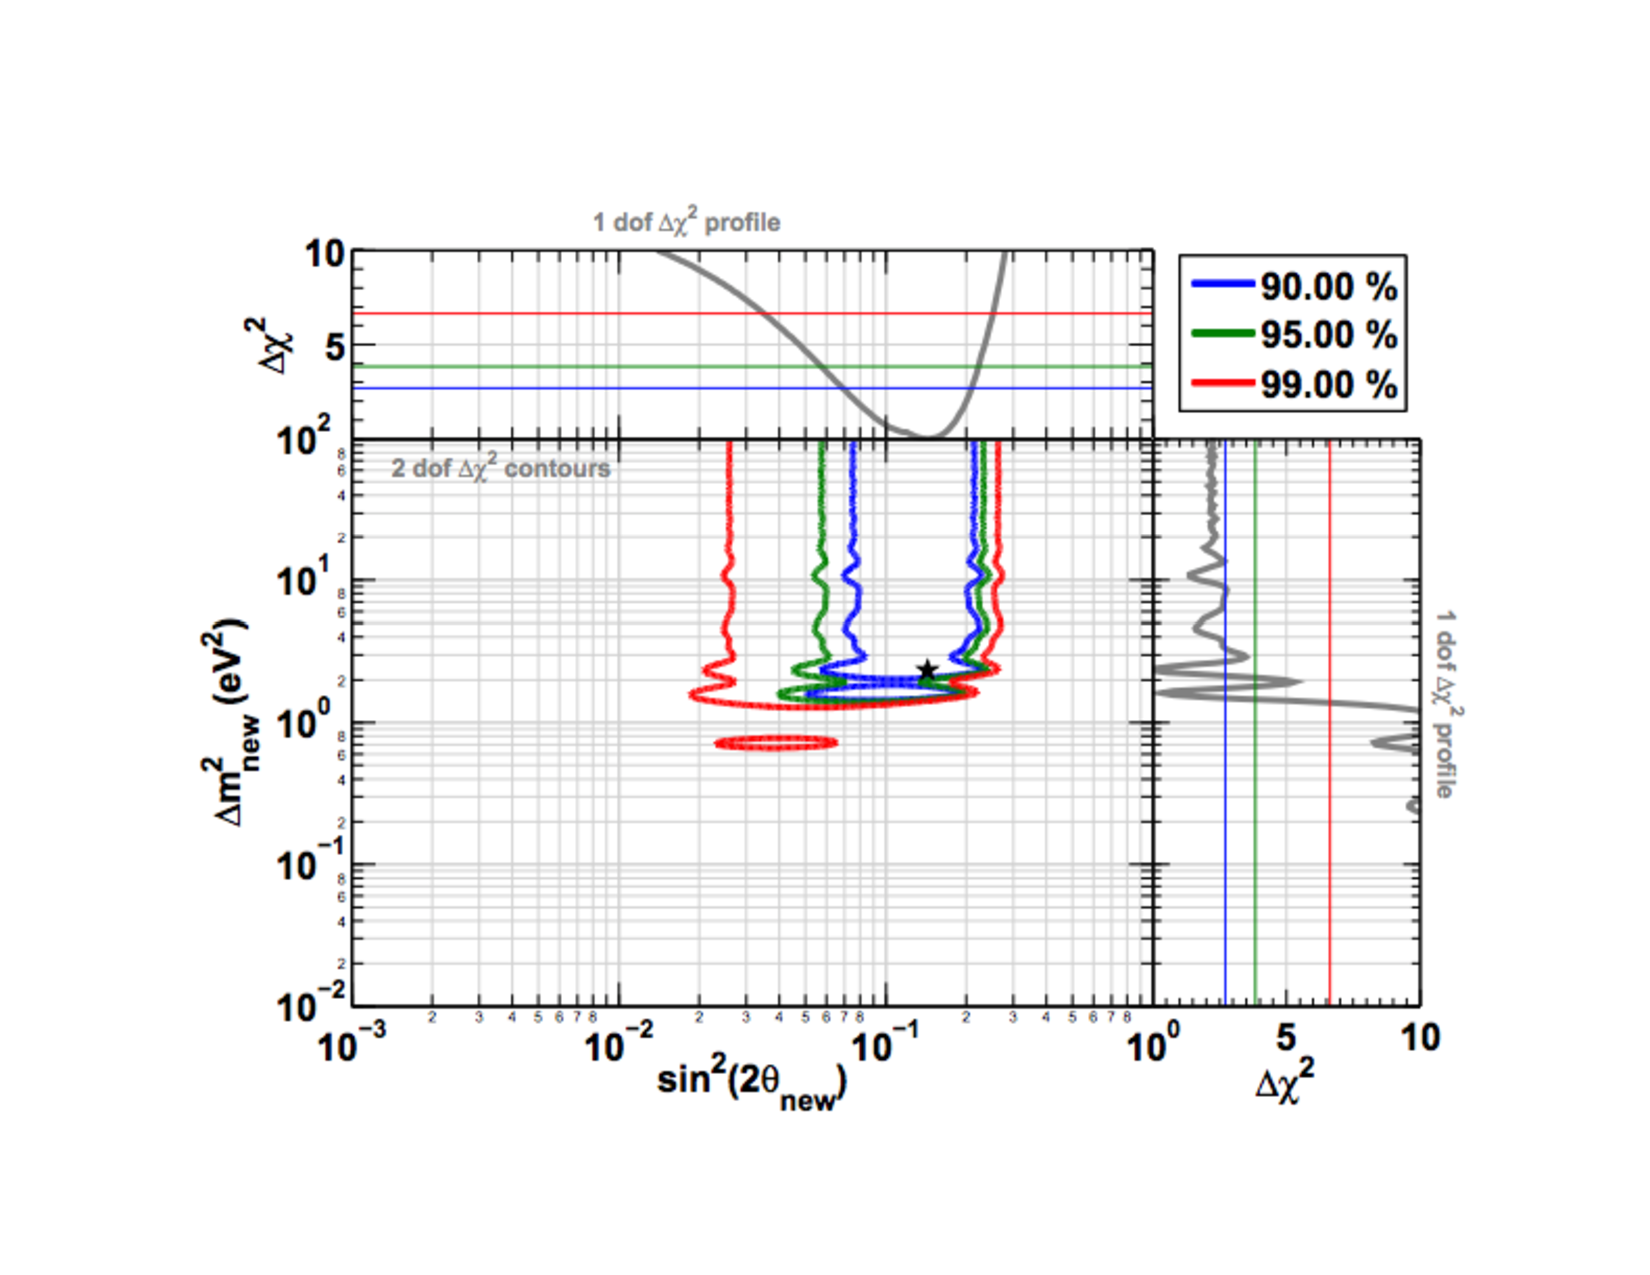
\includegraphics[width=0.7\linewidth]{tex/3-reactorneutrinos-images/RAA_BestFitPoint}
	\caption{Allowed regions in the $\sin^2(2\theta_{14})-\Delta m^2_{14}$ plane resulting from a fit of the 3+1 neutrino model to results from reactor neutrino experiments, SAGE and GALLEX, MiniBooNE, and spectrum measurements from ILL. This global fit results in the constraints $\Delta m^2_{14} > 1.5 \textrm{eV}^2$ and $\sin^2(2\theta_{14}) = 0.14 \pm 0.08$ \cite{Mention:2011rk}.}
	\label{fig:raabestfitpoint}
\end{figure}

If these anomalies are taken as evidence of short-baseline oscillations of electron neutrinos, the simplest way to explain these discrepancies is to add onto the standard model using the 3+1 oscillation model in which there are three active neutrinos and one sterile. This would introduce three new mixing angles, $\theta_{14}$ being the one of interest in reactor neutrino experiments.
A global fit of this model to neutrino data, including results from reactor experiments, SAGE and GALLEX, MiniBooNE, and spectrum measurements from ILL, results in oscillation constraints $\Delta m^2_{14} > 1.5 \textrm{eV}^2$ and $\sin^2(2\theta_{14}) = 0.14 \pm 0.08$, as shown in Figure~\ref{fig:raabestfitpoint} \cite{Mention:2011rk}.


An alternative explanation is that the flux predictions are incorrect and have larger uncertainties than those currently applied. 
The idea that the calculated reactor antineutrino flux is not well understood is bolstered by results from Daya Bay \cite{DayaBayAnomaly}, RENO \cite{Seo:2016uom}, and Double Chooz \cite{DoubleChooz:2019qbj} in which a ``bump" was observed in the experimentally measured antineutrino energy spectrum relative to the model spectrum, shown in Figure~\ref{fig:spectrums}.

\begin{figure}[t]
	\centering
	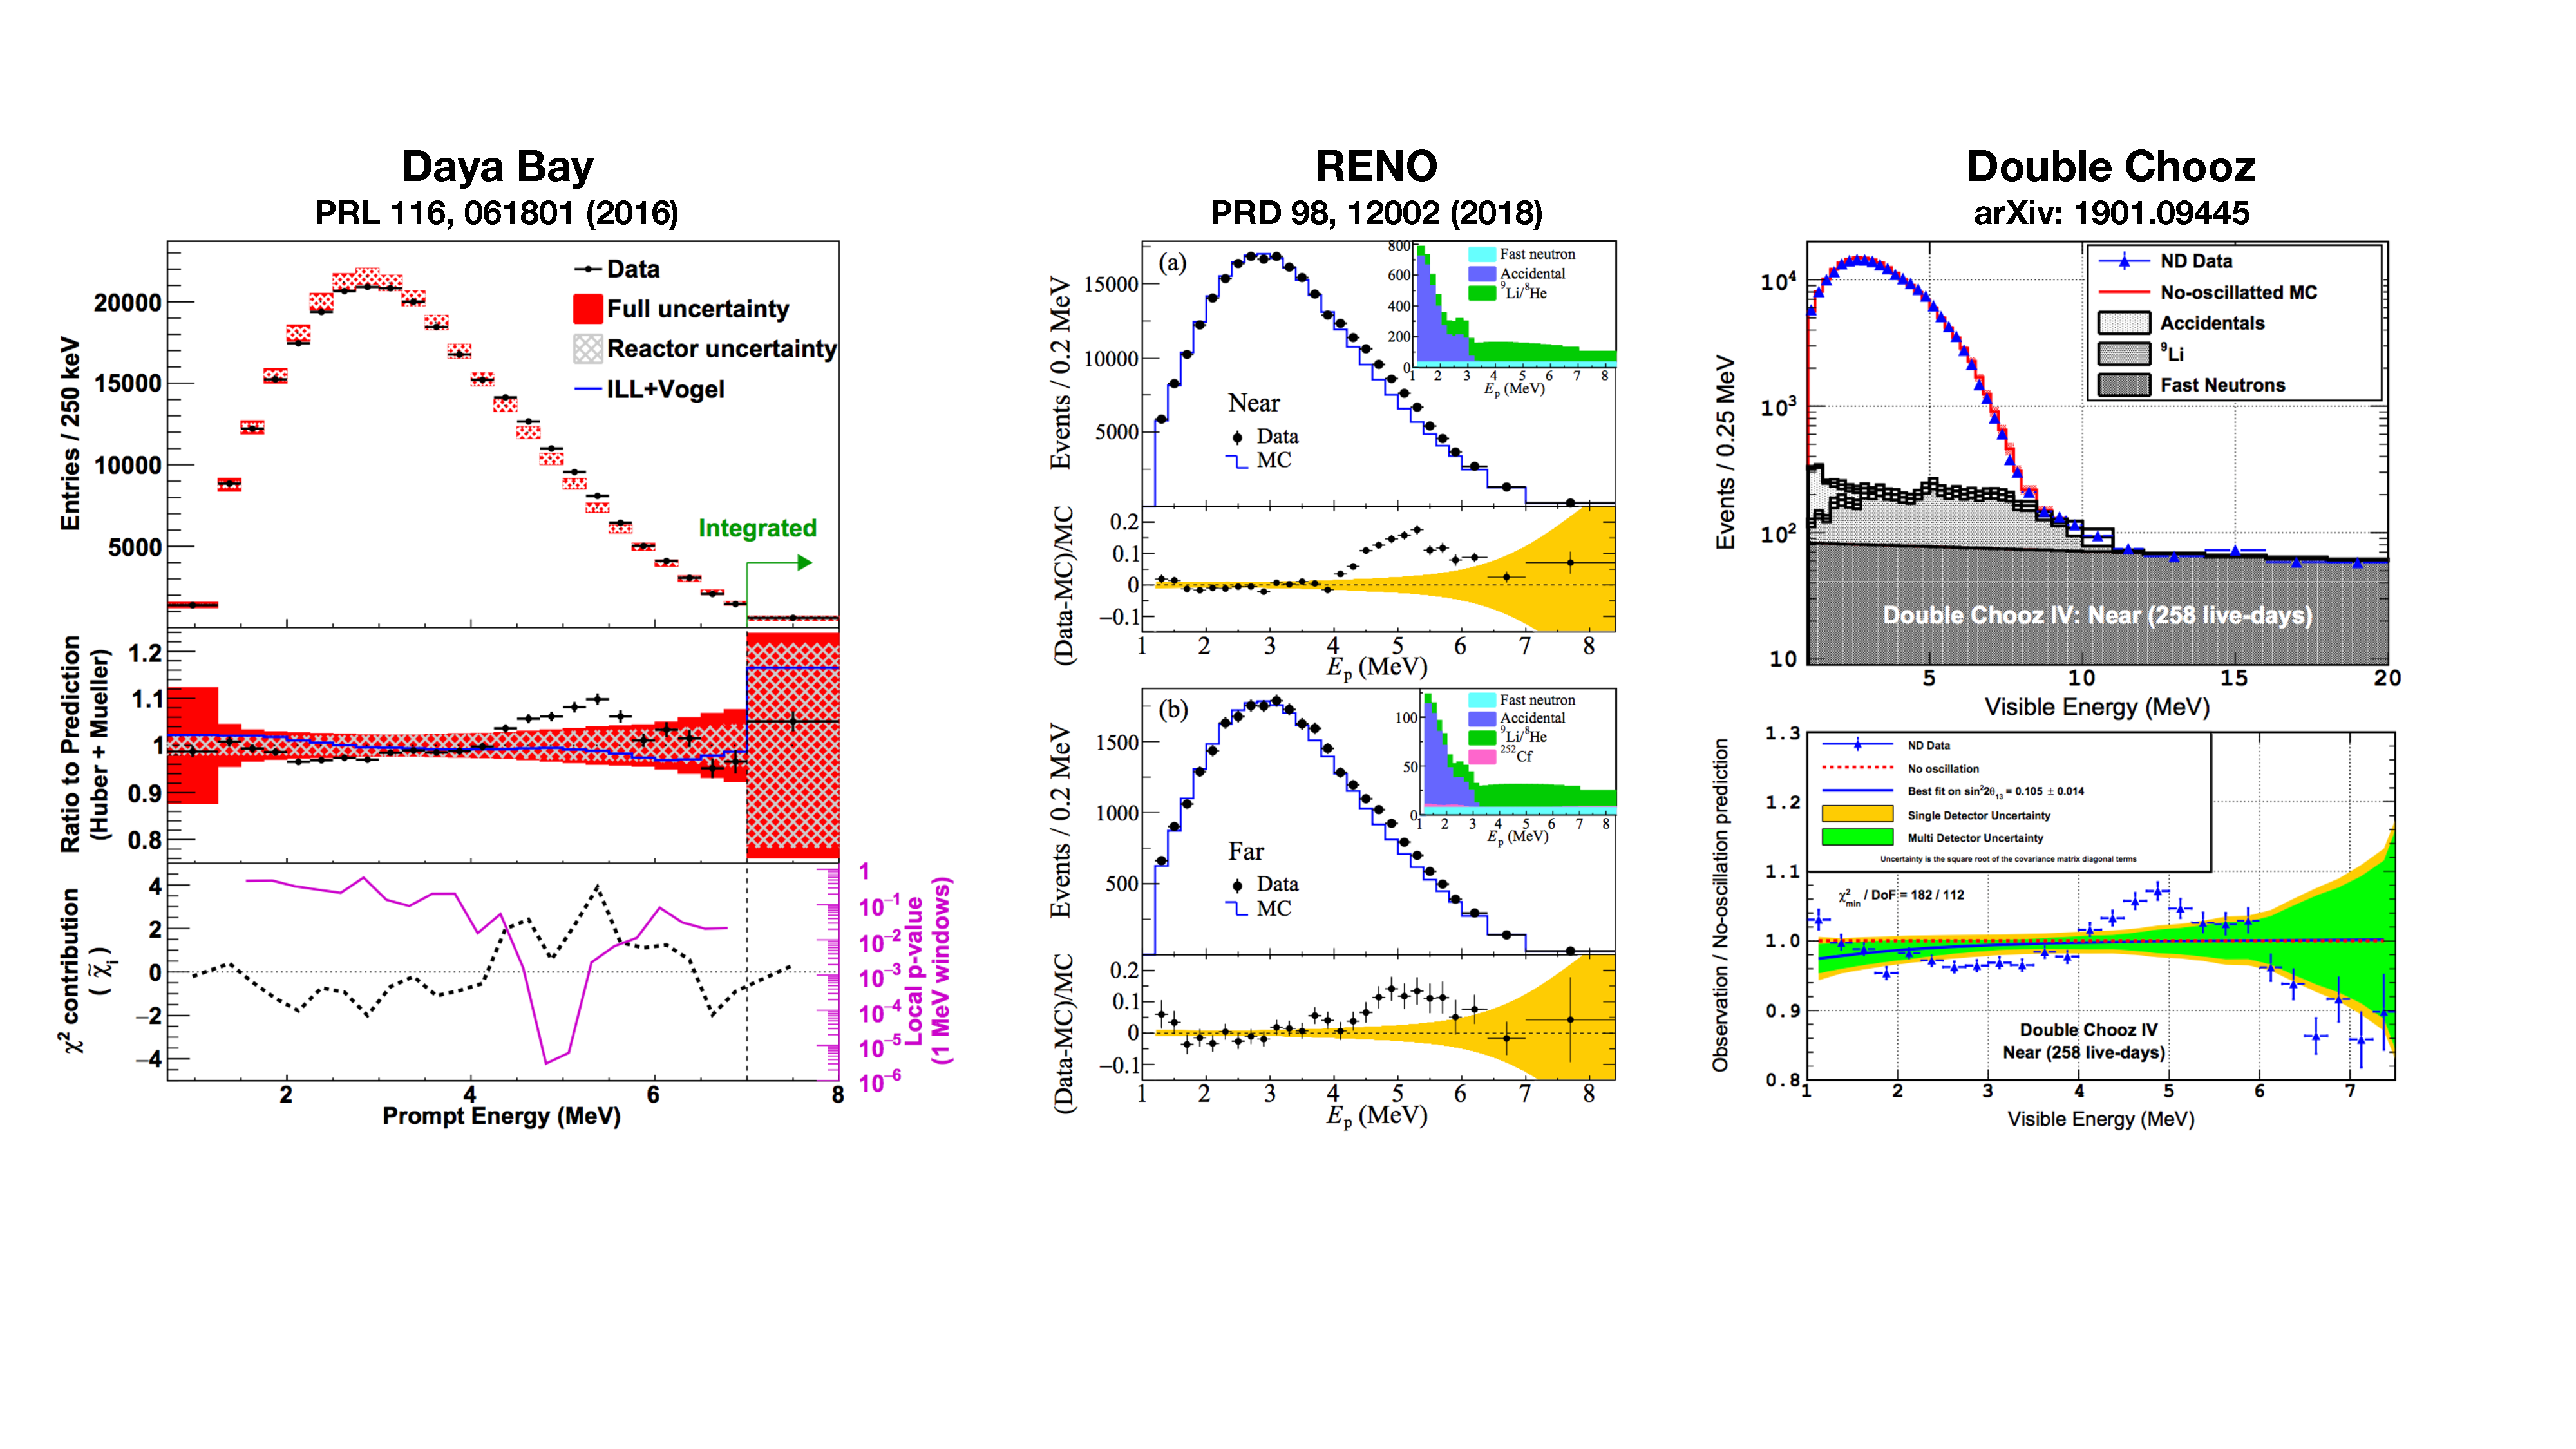
\includegraphics[width=1\linewidth]{tex/3-reactorneutrinos-images/Spectrums}
	\caption{A comparison between the predicted and measured prompt energy spectra of IBD events in Daya Bay \cite{DayaBayAnomaly}, RENO \cite{Seo:2016uom}, and Double Chooz \cite{DoubleChooz:2019qbj}. All experiments observe an excess of events above uncertainty in the model spectrum in the 4-6 MeV region.}
	\label{fig:spectrums}
\end{figure}

In an effort to better understand what aspect of the reactor $\bar{\nu_{e}}$ model is causing the disagreement from data, Data Bay measured changes in the reactor antineutrino flux and spectrum as a function of reactor fuel evolution \cite{An:2017osx, PhysRevLett.123.111801}.
As a reactor burns fuel the relative fraction of fission isotopes $^{235}$U, $^{238}$U, $^{239}$Pu, and $^{241}$Pu in the core changes.
Antineutrino fluxes and spectra differ depending on the fission isotope that is producing the antineutrinos, so, as the reactor runs the $\bar{\nu_{e}}$ spectrum is changing. 

By measuring the evolution of the IBD energy spectrum Daya Bay concluded that incorrect predictions of the $^{235}$U flux may be the primary contributer to the reactor antineutrino anomaly. 
They disfavored a model in which there is an equal deficit from all reactor fission isotopes, implying the existence of a sterile neutrino, at 2.6$\sigma$.
These results were also confirmed by a similar study completed by RENO \cite{PhysRevLett.122.232501}.
Whether the reactor antineutrino anomaly can be solved by the addition of a sterile neutrino, more accurate reactor flux models, or a combination of both is a topic of great interest in the neutrino community and several experiments have been designed to address this matter.
